\chapter{Modelo GRAND}
\label{cap:grand}

No modelo GRAND são tratados três aspectos do gerenciamento de dados: transferência automática dos dados de entrada para o local onde o arquivo será necessário; o envio de resultados é controlado evitando congestionamento da rede; priorização de localidade no disparo de tarefas para não haver transferências desnecessárias de dados degradando o desempenho. Através de uma hierarquia de gerenciadores (Figura 1) é feito o disparo e controle das aplicações. o \emph{Application Manager} (AP) recebe uma submissão de aplicação através de um usuário, os APs mandam os \emph{Submission Managers} (SM) descrições de tarefas assim, sob demanda, são instanciados os \emph{Task Managers} (TM) para controlar a submissão de tarefas a escalonadores de domínios específicos da grade, esses escalonadores recebem requisições dos TMs fazendo a execução das tarefas propriamente ditas.

Pelo fato de que, na atualidade, ambientes grades envolvem principalmente instituições de ensino em aplicações usualmente classificadas como aplicações científicas, o escopo do GRAND é limitado as seguintes itens. 

\begin{enumerate}
    \item heterogeneidade, lembrando que isto afeta diretamente a política de escalonamento por necessitar de saber as características distintas de hardware e software; 
    \item grande número de submissão de tarefas, referindo-se a aplicações que geram centenas ou milhares de processos; 
    \item ausência de comunicação por troca de mensagens, pelo fato da necessidade de inúmeros aspectos nas fases de agrupamento e mapeamento serem considerados; 
    \item interdependência de tarefas, devido ao compartilhamento de arquivos; 
    \item manipulação de grande número de arquivos pelas tarefas; 
    \item o uso de arquivos grandes, através de técnicas como \emph{staging} e \emph{caching}, minimizando a perda de desempenho em função da latência de transmissão; 
    \item segurança, assume-se que exista uma conexão segura entre os nós da grade; 
    \item descoberta dinâmica de recursos; 
    \item gerenciador de recursos local em cada nó; 
    \item uma tarefa é executada em um RMS até sua finalização;
\end{enumerate}

\begin{figure}[htb]
\begin{center}
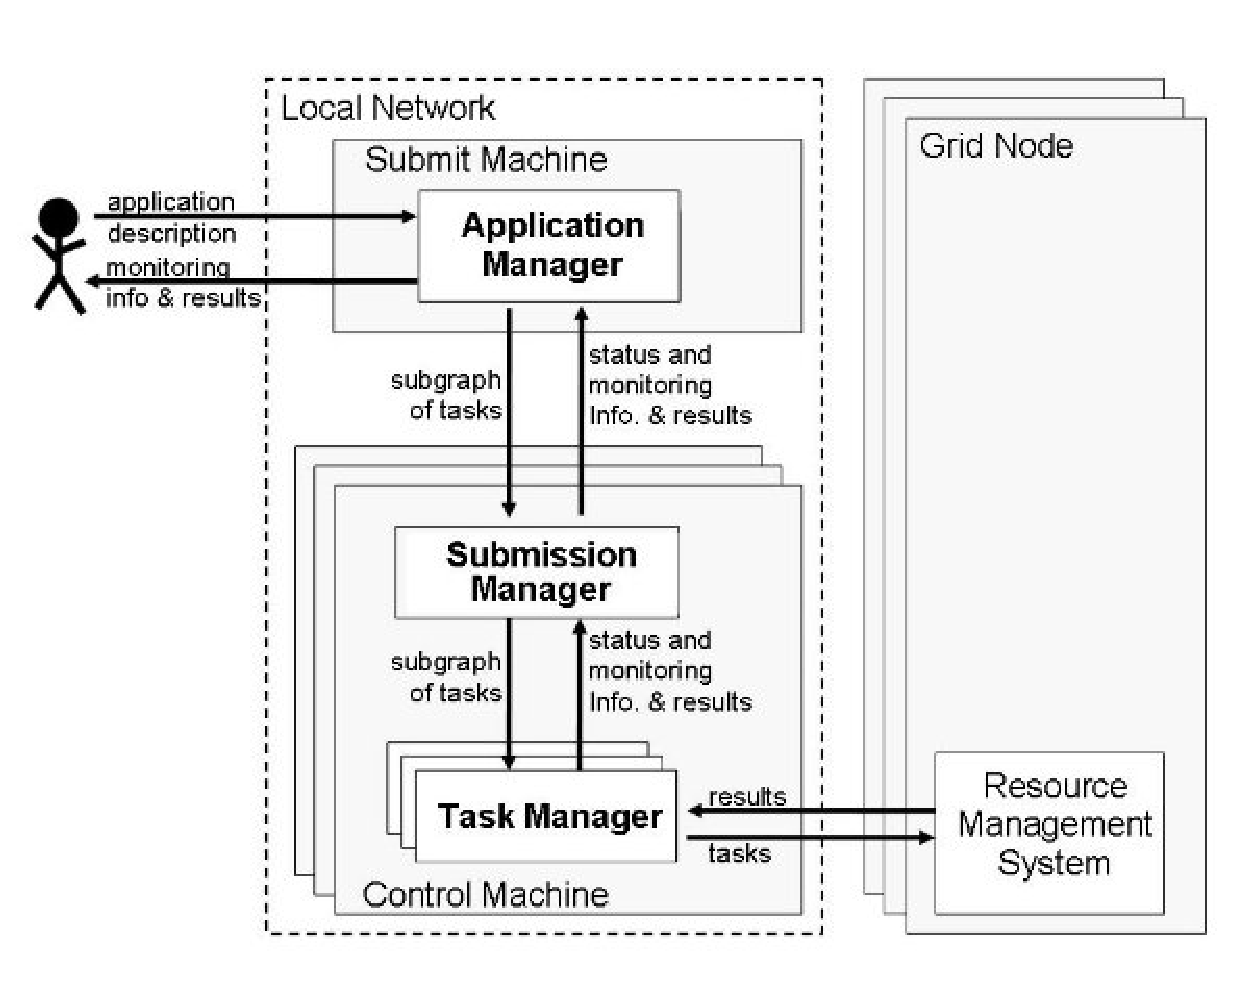
\includegraphics[scale=0.7]{./img/grand.eps}
\caption{Principais componentes do modelo hierárquico de gerenciamento de tarefas}
\label{fig:Modelo_Grand}
\end{center}
\end{figure}
